% PLEASE FOLLOW POSTED GUIDELINES!!

% Please see the two LAr CDR 'guidelines' writeboards in basecamp
% at https://lbne-doc.basecamphq.com/projects/4264323/writeboards
% One is for text, the other for images and figures 

% Replace the following when the name of the experiment is decided
\newcommand{\LBNE}{[Expt-name] }

%%%%%%%%%%%%%%%%%%%%%%%%%%%%%%%%%%%%%%%%%%%%%%%%%%%%%%%%%%%%%%%%%%%%%%%%
%%%%%%%%%%%%%%%%%%%%%%%%%%%%%%%%%%%%%%%%%%%%%%%%%%%%%%%%%%%%%%%%%%%%%%%%
\chapter{Data Acquisition}
\label{ch:trig}

The scope of the data acquisition (DAQ) subsystem includes the 
design, procurement, fabrication, testing, delivery and installation 
of a combination of custom and commerical electronics modules, (including 
commodity computing and networking hardware), as well as both commercial 
and internally developed software.   

\begin{editornote} 
\begin{center}
{\bf Under construction by Giles: New stuff added, old stuff remains}
\end{center}
\end{editornote}
\begin{editornote} 
Here are Giles's notes on what has happened and still needs doing.

Section 1 is OK.  Section 2 is mostly OK, but need a bit more careful
time to make sure the numbers for channel counts are correct and
include the correct rate calcuiations for the new APAs (and remove
reference to zero suppression inside).  Section 3 is OK, but is so
short(just a table) that it can perhaps go elsewhere?  Section 4 and 5
can be merged into one (COBs), the old text is still present and needs
deleting once any nice sentences have been harvested from it.  The
section on artdaq needs augmenting with a full description of the LBNE
implementation with the dual trigger schemes.  The section on timing
isn now too long, but many of the bits are very good and may need
moving elsewhere.  There should be a section on global triggering (of
detectors in several distinct detector halls, and a secion on
supernova triggering.
\end{editornote}

\section{Introduction}
The DAQ subsystem will perform the primary functions of:

\begin{itemize}
  \item Readout of raw data from the LArTPC and other detector
    subsystems,

  \item Filtering and assembly of data into sections which are to be
    treated by the offline reconstruction as a single event, and
    logging to persistent storage media,

  \item Receiving, and using the \LBNE beam-spill signal, 

  \item Configuration, online calibration/checkout, and control of 
        operations of detector subsystems, including the generation 
        and distribution of timing and control signals,

  \item Control of, and readout of data from, devices 
        providing real-time information on detector, subsystem 
        and environmental conditions, and  

  \item Providing user/operator interfaces for these functions via 
        a run control system.
\end{itemize}

A reference design for the DAQ subsystem is presented in this chapter.   
The development of this design is guided by recent experience gained 
in the development of relevant systems for the NO$\nu$A~\cite{novatdr} 
and MicroBooNE~\cite{microboonecdr} experiments, as well as from 
running experiments with comparable channel counts and/or experimental 
conditions, such as D-Zero, CDF, MINOS and ICARUS.  Guidance is also
being obtained during the design and operation of the LBNE 35t
prototype and the futute CERN testing program.

%\section{Description}

The DAQ subsystem is to be located external to the cryostat vessel,
with components in the detector halls and in an on-site control room.
The interfaces are with the front-end electronics for the LArTPC and
photon-detector subsystems.  To increase robustness and up-time, there
is a comparitively loose coupling between the DAQ subsystems in each
detector hall, to allow calibration or maintenence to proceed in one,
while data collection continues in the others.  The DAQ subsystem
interfaces with the Fermilab Accelerator complex (the beam-spill
signal), and has a read-only interface with the cryogenics subsystem
for logging of conditions.  

%\fixme{A pgraph on what DAQ DOES include, first?} I moved the following up from further down.

\begin{cdrfigure}[DAQ subsystem block diagram]{daq15_main}{Block diagram layout of the main
    components of the DAQ subsystem.}
\begin{tikzpicture}[
  every matrix/.style={ampersand replacement=\&,column sep=0.4cm,row sep=0.6cm},
  to/.style={->,>=stealth',shorten >=1pt,semithick,font=\sffamily\footnotesize},
  data/.style={thick},
%  box/.style={draw,thick,rounded corners,fill=yellow!20,inner sep=.3cm},
  box/.style={draw,inner sep=.1cm},
  boxa/.style={box,align=center}]

% Lay the nodes out using a matrix
  \matrix{   
% 1st row
  \node[boxa] (ce) {Cold\\Electronics};
 \&
 \& \node[boxa] (rce) {COB\\LArTPC data\\processors};
 \&
 \& \node[boxa] (trigfe) {Trigger\\frontend\\Computers};
 \& \node[boxa] (trigbe) {Trigger\\backend\\Computers}; \\

% 2nd row
 \& \node[box,inner sep=0.4cm] (fthru) {}; 
 \& \node[boxa] (time) {Time\\Sync};
 \&
 \& \node[boxa] (sc) {Slow\\Control};
 \& \\

% 3rd row
  \node[boxa] (pd) {Photon\\Detectors};
 \&
 \& \node[boxa] (ssp) {SSP\\Photodetector\\digitizers};
 \&
 \& \node[boxa] (datafe) {Data\\frontend\\Computers};
 \& \node[boxa] (databe) {Data\\backend\\Computers}; \\
 };

\coordinate (fthruWL) at ($ (fthru.south west)!0.3!(fthru.north west) $);   % West Low edge of fthru 
\coordinate (fthruWH) at ($ (fthru.south west)!0.7!(fthru.north west) $);   % West High edge of fthru 
\coordinate (fthruEL) at ($ (fthru.south east)!0.3!(fthru.north east) $);   % East Low edge of fthru 
\coordinate (fthruEH) at ($ (fthru.south east)!0.7!(fthru.north east) $);   % East High edge of fthru 

\coordinate (trigfeWL) at ($ (trigfe.south west)!0.3!(trigfe.north west) $);   % West Low edge of trigfe 
\coordinate (trigfeWH) at ($ (trigfe.south west)!0.7!(trigfe.north west) $);   % West High edge of trigfe
\coordinate (datafeWL) at ($ (datafe.south west)!0.3!(datafe.north west) $);   % West Low edge of datafe
\coordinate (datafeWH) at ($ (datafe.south west)!0.6!(datafe.north west) $);   % West High edge of datafe

\coordinate (rceEL) at ($ (rce.south east)!0.3!(rce.north east) $);  % East low edge of RCE 
\coordinate (rceEH) at ($ (rce.south east)!0.7!(rce.north east) $);
\coordinate (sspEL) at ($ (ssp.south east)!0.3!(ssp.north east) $);  % East low edge of SSP
\coordinate (sspEH) at ($ (ssp.south east)!0.8!(ssp.north east) $);

\coordinate (rceSR) at ($ (rce.south)+(0.7cm,0) $);  % South right edge of RCE 
\coordinate (sspNR) at ($ (ssp.north)+(0.7cm,0) $);  % North right edge of RCE 
\coordinate (scWL) at ($ (sc.south west)!0.3!(sc.north west) $);  % West low edge of SC 
\coordinate (scWH) at ($ (sc.south west)!0.7!(sc.north west) $);  % West high edge of SC 

\draw[data] (ce) -| ($(fthruWH)-(0.1cm,0)$) -- (fthruWH);
\draw[data] (pd) -| ($(fthruWL)-(0.1cm,0)$) -- (fthruWL);
\draw[data] (fthruEH) -- ($(fthruEH)+(0.1cm,0)$) |- (rce);
\draw[data] (fthruEL) -- ($(fthruEL)+(0.1cm,0)$) |- (ssp);

\draw[data] (rceEH) -- ($ (rceEH)+(0.5cm,0) $) |- (trigfeWH); 
\draw[data] (rceEL) -- ($ (rceEL)+(0.5cm,0) $) |- (datafeWH); 
\draw[data] (sspEH) -- ($ (sspEH)+(0.55cm,0) $) |- (trigfeWL); 
\draw[data] (sspEL) -- ($ (sspEL)+(0.55cm,0) $) |- (datafeWL); 

\draw[data] (trigfe) -- (trigbe);
\draw[data] (datafe) -- (databe);

\draw[data,dashed] (time) -- (rce);
\draw[data,dashed] (time) -- (ssp);

\draw[data,dashed] (scWH) -| (rceSR);
\draw[data,dashed] (scWL) -| (sspNR);

\draw[data,dotted] (fthru.north) -- ($(fthru.north)+(0,2.7cm)$) node [left] {In cryostat} node [right] {Room temp.};
\draw[data,dotted] (fthru.south) -- ($(fthru.south)-(0,2.7cm)$);

\end{tikzpicture}
\end{cdrfigure}
The DAQ subsystem reference design described in this chapter is shown
in figure~\ref{fig:daq15_main} and consists of the following
components:
\begin{itemize}
  \item custom "Cluster-on-Board" (COB) digitised data processing
    modules, residing in ATCA crates located in the detector hall to
    receive data from the LArTPC (transmitted via redundant high-speed
    link) and to carry out data merging and data compression (see
    section~\ref{sec:daq_cob})
  \item custom `SSP photon detector digitizers' which digitize and
    process the light signals (described in section~\ref{sec:pd_ssp}) 
  \item two local farms of commodity computers providing two separate
    branches of readout, triggering, event processing and logging of the
    detector computers; these use the artDAQ toolkit for data
    acquisition systems (see section~\ref{sec:daq_artdaq})
  \item a custom timing system consisting of a master unit, situated
    on the surface, that locks onto a GPS clock and distributes timing
    signals to the data concentrator modules via slave units (see
    section~\ref{sec:daq_timing})
  \item dedicated computer nodes that host run control online
    monitoring, database services and slow controls processes
\end{itemize}
%
The DAQ subsystem does not include power-supply hardware for the
LArTPC or front-end electronics, nor does it include the cryogenics
subsystem process-control and monitoring functions.  The SSP readout
modules for the photon subsystem is in the photon subsystem part of
the project.

\section{Design Considerations}

\subsection{Physics Considerations}

The physics considerations determine the scale of the primary tasks of
digitizing the LArTPC data readout, event building and online
processing.  In addition to rates for processes of interest, the DAQ
subsystem design depends critically on the specifications for the
LArTPC and front-end electronics systems, chosen to satisfy the \LBNE
physics requirements.  As described in Chapter~\ref{ch:tpc}, obtaining
sensitivity to signals that occur independently of the \LBNE beam
spill, such as those from nucleon decay, atmospheric neutrinos or
supernova-neutrino bursts, requires a free-running transmission of
data from the LArTPC front-end electronics.  The sampling rate of
2~MHz has been chosen so as to achieve the required position
resolution along the ionization drift direction.

The task of data transfer is facilitated by multiplexing and utilizing
high-speed data lines (1Gbps) in front-end ASICs in the LAr, and by
redundant data lines that provide connection to data-acquisition
hardware located outside the cryostat.  The hardware receiving the raw
TPC data then can perform zero-suppression and/or data compression, as
desired, and forwarding the sparsified data to a backend processing
farm for event building, reconstruction, and filtering.  
The \LBNE beam-spill signal and data from the photon-detection system
are considered part of the data stream, and can be used at this stage
to select events for processing and storage as desired.

\subsection{Technical Considerations}
In addition to physics considerations, the DAQ design goals include  
minimizing the impact of single-point failures, maximizing the uptime and maximizing 
the use of commercial components.  
For the reference design described here, sited at the 4850L of the Sanford Laboratory, the 
atmospheric-muon rate is small enough -- 0.1~Hz within the full LAr-FD active 
volume -- to contribute only negligibly to the DAQ bandwidth requirement.
%For reference, the rate at the alternate 800L site 
%is estimated to be 500~Hz within the active volume.  
%This and other assumptions are discussed below in 
%Section~\ref{sec:v5-daq-assumptions}.  
The requirements on the DAQ system are listed in the
requirements documentation~\cite{lar-fd-req}.

\subsection{Event Rates and Timing}
\label{sec:v5-daq-assumptions}

%The DAQ subsystem design depends on assumptions pertaining to physics goals as well as detector configuration and conditions. 

Signals associated with beam events will be localized within the 
LArTPC and synchronous with discrete (${\cal O}(1\,s)$ rep rate) 
beam-spill intervals spanning 
approximately $10\,\mu s$.  
However other physics events of interest will occur at random 
times, and can be dispersed throughout the TPC volume as in the case 
of neutrino bursts from supernovae.  Other specific signatures, such 
as very slow-moving magnetic monopoles ($\beta < 10^{-3}$) may involve 
signals spanning sample times exceeding the 2.3-ms maximum ionization-drift time.  

Cosmic-ray muons dominate the physics rate, even at the proposed 4850L site.  
However, this rate is negligible with respect to noise sources.  The
reference design proposed here would be capable of operation at
shallower depths, up to about the 800L, without sgnificantly impacting
the design.

\fixme{Update these next two paragraphs, remove references to zero
  suppression in cold}
 As described earlier in this report
(see Figure~\ref{fig:tpc-elec-schematic}), 
the cold electronics for a single Anode Plane Assembly 
will consist of twenty 128-channel Front-End Readout 
Boards, each providing a single digital input to a 20-channel
Data Output Board, which includes a 20$\times$ MUX stage into a  
driver for a redundant pair of LVDS outputs.   

The Front-End Boards will generate non-zero-suppressed data: worst-case 
scenarios (i.e., $>10\,$GeV EM showers contained within a single APA) 
indicate roughly a factor of ten reduction in the number of samples 
read out with respect to the maximum (2304 wires $\times$ 4625 0.5-$\mu$s 
samples per wire).  

For cosmic-ray muons, the rejection factor is estimated to be $\sim 200$.  
The rejection factor is of course much higher in APAs 
not containing any portion of a physics event.  Radioactive decay 
from $^{39}$Ar and $^{85}$Kr in the LAr, and to a lesser extent from 
detector materials (U/Th/Co/K), is estimated to provide a
65-kHz/APA rate of activity of energy above about 300~keV (0.3 MIPs) 
but less than $\sim 5\,$MeV, while 
electronics noise (assuming 10:1 S/N for 1 MIP, and a threshold of 0.3 MIPs) 
will contribute a relatively low rate per APA of singles.  
Table~\ref{tab:daq-signal-rates} provides a summary of these rate 
estimates.  Work is ongoing to further refine them.
%
\begin{cdrtable}[Rates and data sizes/rates for various processes.]
  {lcccc}{tbl:daq-signal-rates} {Per-APA estimates of rates and
    data sizes/rates for various processes.  Unless otherwise stated,
    estimated numbers of samples and data rates assume suppression of
    signals below 0.3 MIP.  `Inst.\ Data Rate' refers to the number of
    bits in a 2.3-ms long data block divided by this time interval,
    while `Avg.\ Data Rate' factors in the process rate.  A 12-bit ADC
    is assumed, and no allowance is made for data items such as
    time-stamp, channel identifier, etc.}
  
    {\bf Process} & {\bf Rate } & {\bf Samples}
                  & {\bf Inst.\ Data } & {\bf Avg.\ Data}  
                  \cr 
                  & {\bf (kHz/APA)}  & {\bf (per APA)}
                  & {\bf Rate (Mbps)} & {\bf Rate (Mbps)} \cr \hline
    Generic 2.3 ms interval 
                  & 0.43 & $1.06 \times 10^7$ 
                  & 55,000 & 55,000 
                  \cr 
                  (not zero-suppressed) & & & & \cr \hline
    Cosmic ray muons (4850L)
                  &  $6\times 10^{-7}$ & $5 \times 10^4$ 
                  &  260 & $1\times 10^{-4}$
                  \cr 
                  & & & & \cr \hline
    Cosmic ray muons (800L)
                  &  0.0034 & $5 \times 10^4$ 
                  &  260 & 2.0 
                  \cr 
                  & & & & \cr \hline
    10 GeV EM shower 
                  &  --- & $1 \times 10^6$
                  & 5,200  & --- 
                  \cr
                  & & & & \cr \hline
    Radioactivity: $\gamma$: U/Th
                  & $\sim 1$ & 40
                  & 0.48  & 0.48
                  \cr
    \phantom{Radioactivity:} $\beta$: $^{39}$Ar, $^{85}$Kr
                  & 63 & 24
                  & 18  & 18
                  \cr
                  & & & &  \cr \hline
    Electronics noise
                  & $\sim 1$ & 15 
                  & 0.2  & 0.2 
                  \cr 
                  (not common mode) & & & & \cr \hline
\end{cdrtable}

It can be concluded from the table that the average data rates out of the 
front-end electronics system are manageable: 
about 20 Mbps of `salt and pepper' per APA 
due to radionuclides in the Ar and TPC materials. 
Large beam- or atmospheric-neutrino interactions or 
showering ultra-high-energy cosmic-ray muons will result in high (Gbps-level)
instantaneous rates on the scale of the maximum ionization drift period, 
but contribute negligibly to the average rate.

\fixme{Update this section}
With sufficient buffering in front-end ASICs, as described 
in Chapter~\ref{ch:tpc}, the plan of having a single LVDS output line per APA 
(plus a second one for redundancy) is easily realizable.  However, 
to be conservative, and to provide opportunities for collecting data with 
relaxed zero-suppression, the DAQ reference design described below 
allows for as many as 20 output lines per APA (one per front-end board), 
each operating below 24~Mbps.  This leads to a capacity for APA output 
rates up to 480~Mbps, well above the $\sim 20$ Mbps expected. 

%%%%%%%%%%%%%%%%%%%%%%%%%%%%%%%%%%%%%%%%%%%%%%%%%%%%%%%%%%%%%%%%%%%%%%%%
%%%%%%%%%%%%%%%%%%%%%%%%%%%%%%%%%%%%%%%%%%%%%%%%%%%%%%%%%%%%%%%%%%%%%%%%
\section{Architecture Summary}
\label{sec:v5-trig-daq}

The reference design of the DAQ system is summarized in 
block diagram form in Figure~\ref{fig:daq15_main}.  
Component counts are given in Table~\ref{tab:daq15_component_counts}.\
%
%\begin{figure}[htbp]
%\centering
%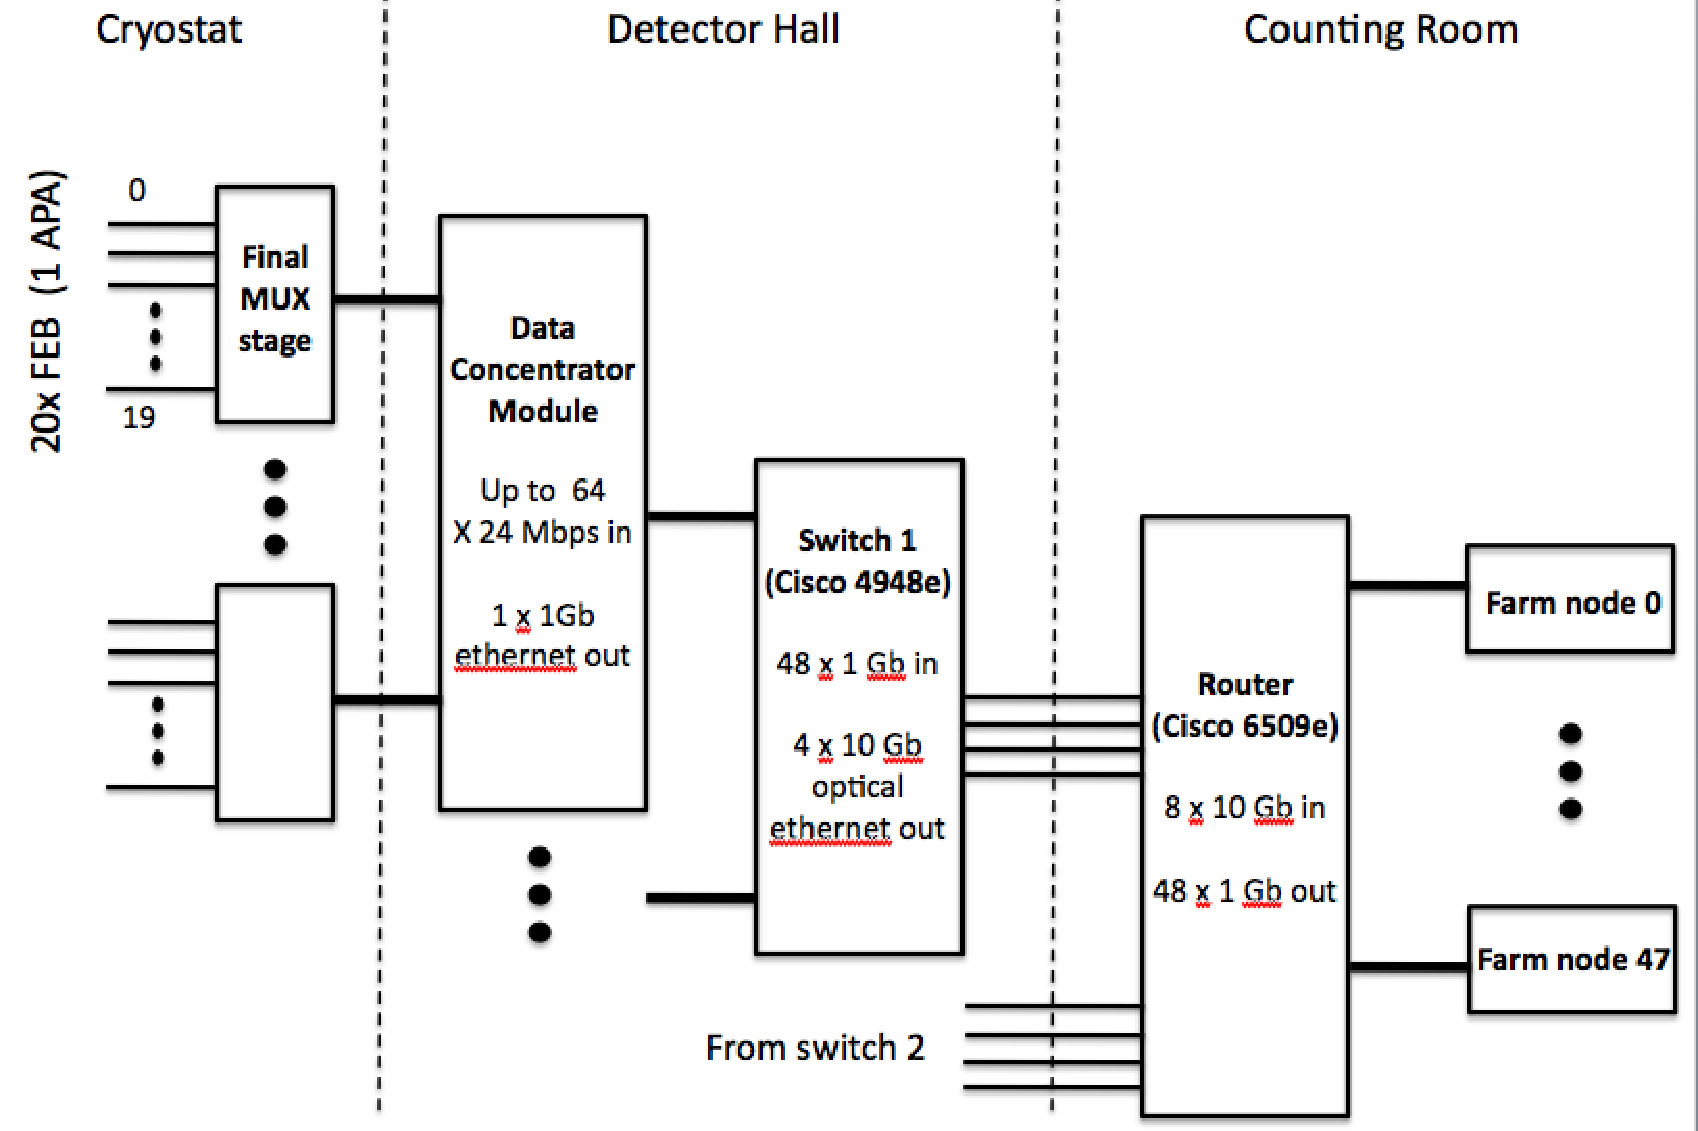
\includegraphics[width=\linewidth]{v5c4-daq-block-diagram}
%\caption{Block diagram depicting the DAQ reference-design architecture}
%\label{fig:daq-block-diagram}
%\end{figure}
%
\begin{editornote}
Update the entries in the table.  Be precise about how many items are
needed and for what sized detector.
\end{editornote}

\begin{cdrtable}[DAQ subsystem component counts]{ll}{daq15_component_counts}
  {DAQ subsystem component counts for one 20-kton module/cryostat.
    The total component count for the two-cryostat LAr-FD will be
    twice what is shown.}
    {\bf Quantity} & {\bf Description} \\
   60  &  COBs (Cluster on Board) each with 8 RCEs\\
   20  & 2-slot ATCA Shelves  \\
   2   & Ethernet Switches   \\  
   60  &  TPC Readout Compute Nodes \\
   1   &  Master Timing Unit with GPS Receiver\\
   10  &  Slave Timing Units  (assuming we build new, improved ones) \\
   8   &  Event Builder Compute Nodes  (???) \\
   8   &  Software Filter Compute Nodes (???) \\
   1   &  Run Control Compute Node   \\
   1   &  Slow Control Compute Node   \\
   1   & DAQ Database  Compute Node   \\
\end{cdrtable}

%%%%%%%%%%%%%%%%%%%%%%%%%%%%%%%%%%%%%%%%%%%%%%%%%%%%%%%%%%%%%%%%%%%%%%%%
%%%%%%%%%%%%%%%%%%%%%%%%%%%%%%%%%%%%%%%%%%%%%%%%%%%%%%%%%%%%%%%%%%%%%%%%
\section{COB - Cluster on board modules}
\label{sec:daq_cob}

The primary interface between the TPC front-end electronics (FE) and
the DAQ subsystem consists of an ATCA-based system of RCEs
(Reconfigurable Cluster Elements).  The RCE system receives the
serialized raw data for the FE, performs zero-suppression on it, and
packetizes and transmits the resulting sparsified data to a back-end
data farm for event building and further processing.  Additionally,
the RCE system transmits timing and control signals to the FE as well
as forwarding configuration data to them at start-up.

The RCE system consists the following components: a commercial ATCA
shelf (2-, 6-, or 14-slot), a Cluster-On-Board (COB) which is the
"front board" in ATCA terms, and a Rear-Transition-Module (RTM) which
is the "rear board".  The COB is a custom board, developed by SLAC,
which holds the processing power of the system.  The COB (see Figure
\ref{fig:daq15_cob}) consists of 5 bays for holding daughter boards, an onboard
10-GbE switch, and both 10- and 1-Gb ethernet connections for
communications with the back-end system.  Four of the daughter-board
bays are for Data Processing Modules (DPM), each of which can hold up
to two RCEs.  The RCE is the core procession unit of the system; it is
made up of a modern SoC (currently, the Xilinx Zynq-7045) with
multiple high-speed I/O ports (up to 10-Gbps each) and external DRAM
and flash memory controllers.  The other bay on the COB contains the
Data Transmission Module (DTM) which is responsible for distributing
timing and trigger information to and between the DPMs.

While the COB hardware is application agnostic, the RTM is application
specific. The RTM provides the mechanical interface between the
front-end (or, in our case, the flange electronics) and the back-end,
as well as other external sources such as the timing or trigger
systems.  In the case of LBNE, we propose to use fiber optic
connections between the flange and the TPC DAQ using QSFP+ connectors.
Currently, each RTM can accommodate up to 16 QSFP+ connections.

With the assumption that each cold FE board multiplexes it's 128 wire
channels to 4 outputs at 1-Gbps each, the non-zero suppressed data for
1 APA can be fed into a single COB (containing 8 RCEs).  Each RCE
would receive data from 2 FE boards, perform zero-suppression, and
send the result to the back-end.  There are some options regarding the
physical distribution of the shelves.  One option is to have a smaller
shelf at each flange port, each shelf collecting data from the 2- or
4-APAs accommodated by that port.  Alternatively, the fibers from all
APAs could be routed to a central location into a smaller number of
large ATCA-shelves.

\begin{figure}[hbt]
  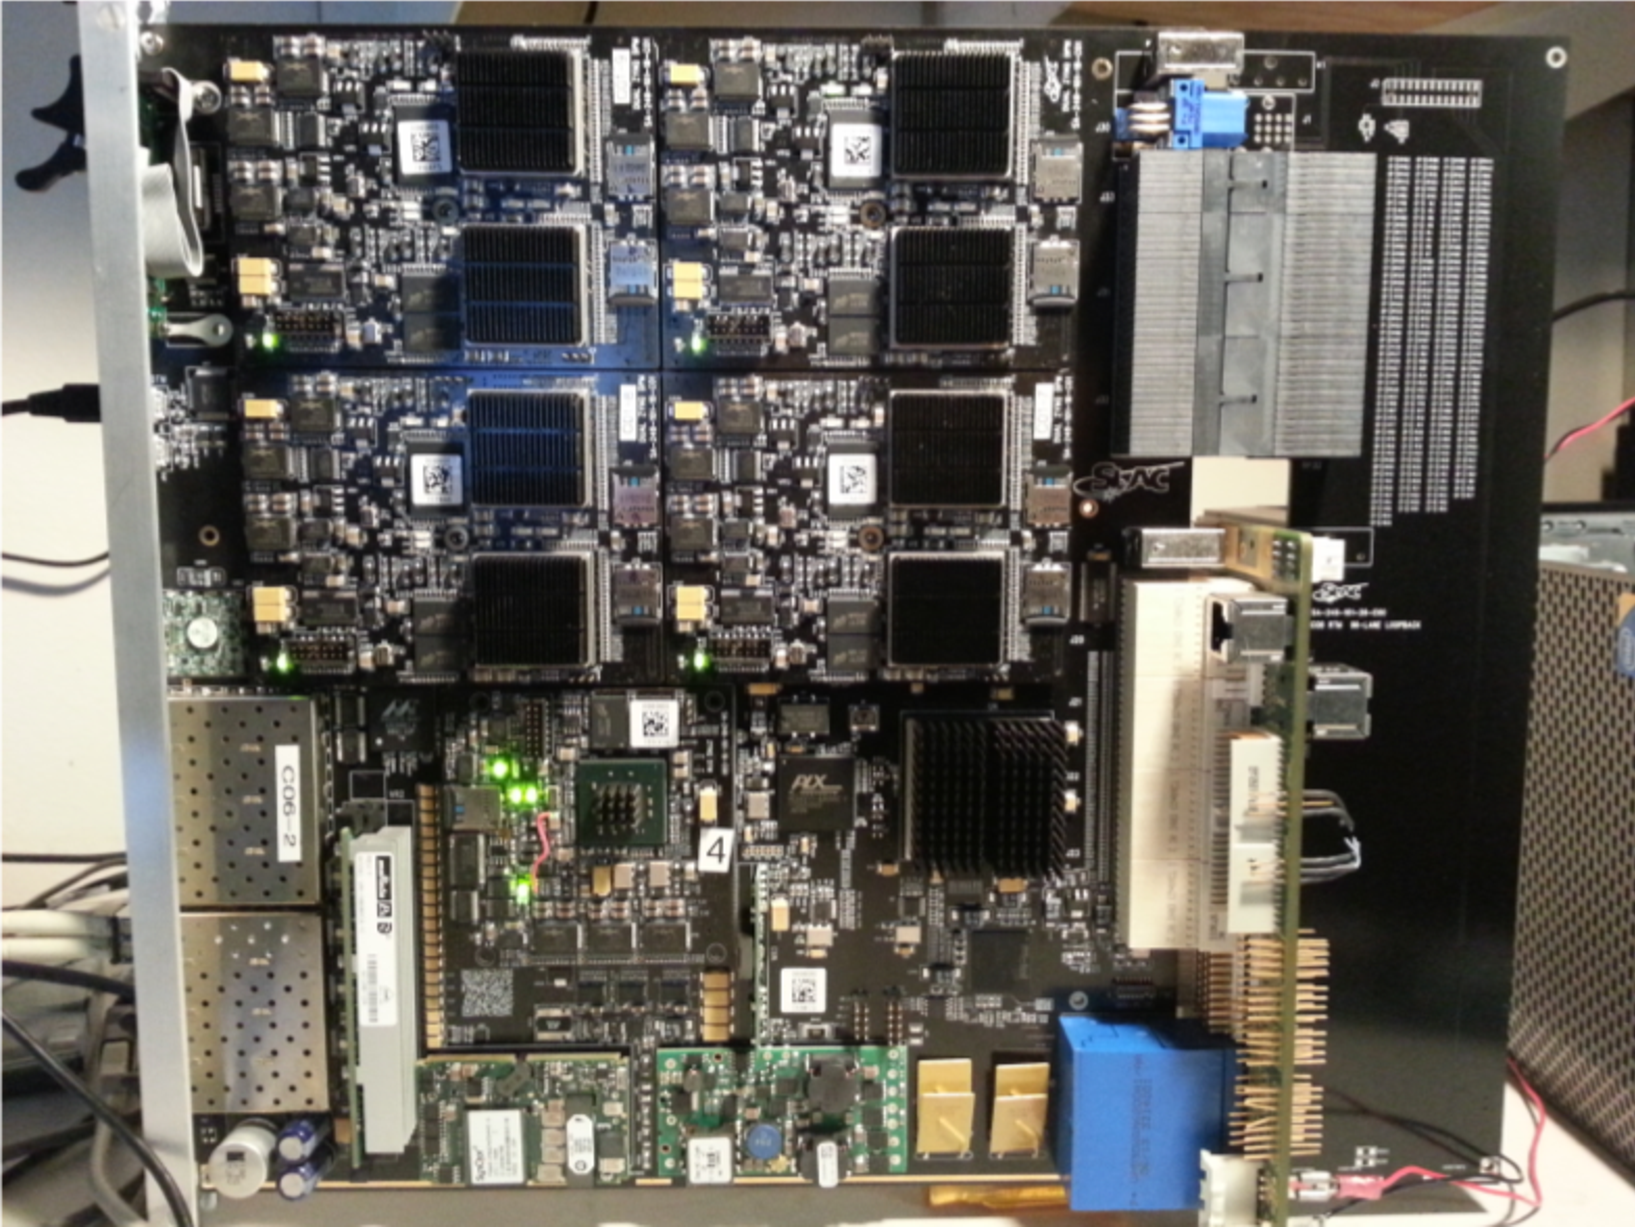
\includegraphics[scale=0.6]{daq15_COB-gen3.pdf}
  \caption{\label{fig:daq15_cob} The COB (left) and RTM (right).  }
\end{figure}
\begin{figure}[hbt]
  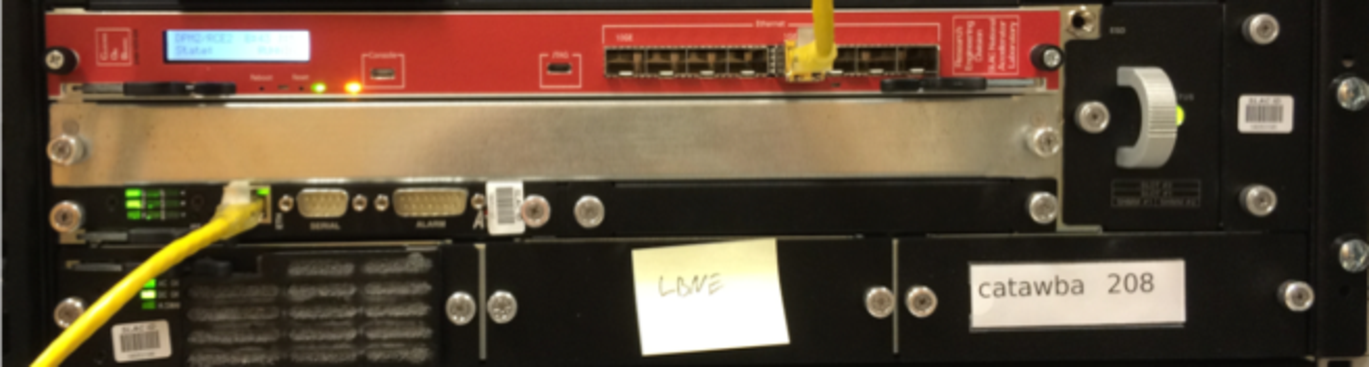
\includegraphics[scale=0.6]{daq15_acta-rtm.pdf}
    \caption{A front view of the ATCA crate with a COB in the top slot. }
\end{figure}

\section{Data Concentrator Module}
\label{sec:v5-trig-datatransfer}

The \LBNE/LArTPC Data Concentrator Module (DCM) serves as the primary interface 
between the cold TPC electronics and the DAQ subsystem, with the main task 
of receiving serial data pushed out of the front end.  It also packetizes and 
transmits the data to `data farm' computers for event 
building via an ethernet switch array, described in 
Section~\ref{sec:v5-trig-switch}.  Finally, it will provide the interface 
for transmitting timing and control signals to the cold electronics. 
As such, it is envisioned to provide the functionality of NO$\nu$A's custom 
electronics module of the same name, and similarly, the digital portion 
of MicroBooNE's ``Front End Module'' (FEM) cards.  

For the purposes of this conceptual design, the NO$\nu$A DCM 
is considered as is.  Several NO$\nu$A prototype modules are shown in 
Figure~\ref{fig:daq-dcm-photo}.  The NO$\nu$A DCM consists of 64 input 
ports (RJ45 sockets), and a single 1~GB output line.  A large 
FPGA provides preliminary data processing capability.  A processor (running 
Linux) provides local control for configuration, buffering and routing 
functions.
%
\begin{figure}[htbp]
\centering
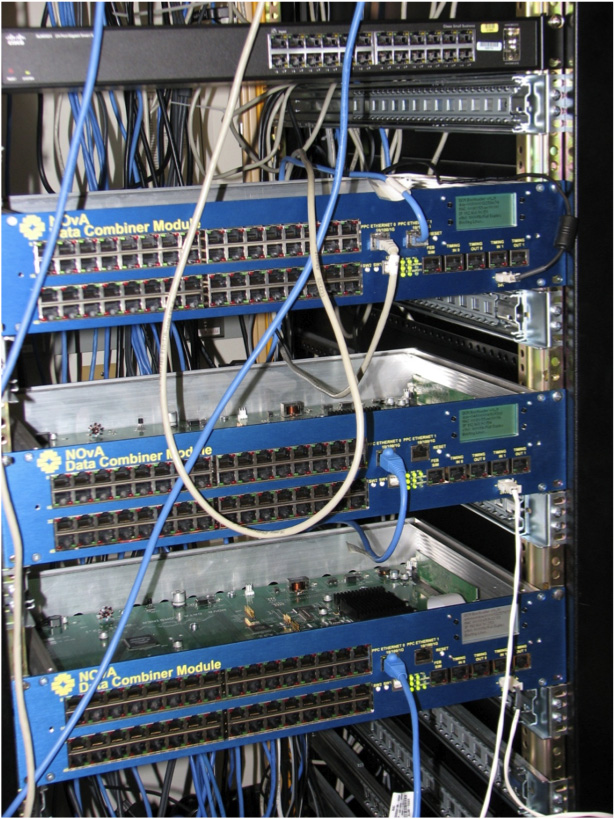
\includegraphics[width=0.4\linewidth]{v5c4-daq-dcm-photo}
\caption{Photograph of several prototype NO$\nu$A Data Concentrator Modules.}
\label{fig:daq-dcm-photo}
\end{figure}

Assuming the Data Output Board is implemented in the cold volume with 
20$\times$ muxing to provide a single output line per APA, only a handful 
of NO$\nu$A-style DCMs would be required to read out the entire detector.  
Considering typical data rates of order 20~Mbps per APA 
(see Table~\ref{tab:daq-signal-rates}), the 1~Gb (80 MB/s) 
DCM output bandwidth 
could comfortably accommodate more than a few APA's.
More likely, the \LBNE DCMs would be designed for fewer input lines 
in this case, in order to distribute them rationally. 

On the other hand, allowing for the possibility of 20 output lines per APA, 
the NO$\nu$A DCM footprint is well matched to the \LBNE APA granularity.  In 
this case, a single DCM could serve two or three APAs.  Outputs from auxiliary 
detector elements could make use of the otherwise unused DCM input channels.
To obtain a conservative estimate of costs, this configuration is considered 
with two APA's per DCM.


\subsection{Data Processing/Handling}
%: demuxing, unpacking, additional zero suppresion} -- too long a title 

As currently imagined, buffers in the front-end electronics will constitute  
a source of variable-length (i.e., zero-suppressed) time-ordered sequence 
of samples for each channel (wire) registering activity, along with a 
channel address and time stamp.  Although this format is likely to be 
suitable for transmission to the data farm, the DCM's task of generating 
ethernet packets also provides an opportunity for additional data processing.  
If re-formatting or additional zero suppression is desired, 
it could be done here.   

\subsection{Timing, Control and Configuration Signals}

The DCM will provide the interface for the transmission of 
timing, control and configuration signals to the TPC/front-end electronics.
More detail on these signals is given in following sections.

%%%%%%%%%%%%%%%%%%%%%%%%%%%%%%%%%%%%%%%%%%%%%%%%%%%%%%%%%%%%%%%%%%%%%%%%
%%%%%%%%%%%%%%%%%%%%%%%%%%%%%%%%%%%%%%%%%%%%%%%%%%%%%%%%%%%%%%%%%%%%%%%%
\section{Ethernet Switch Network}
\label{sec:v5-trig-switch}

The network accomplishing transmission of data from DCMs to the data 
farm will consist of two layers of ethernet switch arrays.  
The first level will reside in the detector hall, and is imagined to be 
able to operate with little external control.  Commercial switch modules 
such as the Cisco 4948E are well suited for this application.  The 4948E 
has 48 1-GB input ports and four 10-GB optical output ports, 
as well as 175~MB of buffer memory.  Two modules will support the 
required data throughput for the entire detector.

The second level will be deployed in the counting room and will 
serve as a router to the data farm nodes located there.  For this application 
the Cisco 6509E switch chassis provides a possible implementation.  This 
would be loaded with a single 8-port 10 GB blade for input data from the 
4948E's, and a single 48-port 10/100/1000~MB blade for 1-GB output to 
farm nodes.

Routing information will be provided to DCMs by a Routing Master.  This 
task will run on a computer located in the counting room.  It will monitor 
the state of data farm nodes, and provide routing information to DCMs.


%%%%%%%%%%%%%%%%%%%%%%%%%%%%%%%%%%%%%%%%%%%%%%%%%%%%%%%%%%%%%%%%%%%%%%%%
%%%%%%%%%%%%%%%%%%%%%%%%%%%%%%%%%%%%%%%%%%%%%%%%%%%%%%%%%%%%%%%%%%%%%%%%
\section{Event Building and Triggering}
\label{sec:v5-trig-evtbuild}

The event building and triggering function of the LAr-FD DAQ system 
will be performed by the data-farm computers.  Event data will be staged 
locally before being transmitted in quasi real-time (nominally to Fermilab) 
for archival to persistent storage. 

\subsection{Artdaq}

The data acquisition software for the 35-ton prototype detector is
based on artdaq which is a toolkit for building DAQ systems.  It has
been developed at Fermilab and is in use in several other experiments.
Within artdaq, core DAQ functions are provided by the toolkit, and
experimenters develop the modules that perform the functions that are
specific to the experiment.  For the 35-ton detector, LBNE
collaborators have developed modules that configure and read out the
COB and SSP boards that are connected to the LArTPC and photon system
detectors, respectively.  Members of the experiment are also
developing reconstruction and filtering software modules that will
analyze the data as it is acquired.  The artdaq-based DAQ system for
the 35-ton detector has been successfully used to acquire data in
electronics and detector integration tests, and artdaq has been the
default choice for the DAQ framework for the full LBNE detector for
some time.  As part of this, a preliminary design has been developed
for the full detector to use a two-stage artdaq system to stream
zero-suppressed data into a farm of processes, run software modules to
find events of interest, and use the results of this software trigger
to initiate the readout of all of the data produced for the events of
interest.

In thinking about the data acquisition system for a reconfigured
long-baseline neutrino experiment, it is recognized that using a
toolkit such as artdaq has advantages in that it allows experimenters
to leverage existing infrastructure and only develop the components
that are necessary for their experiment.  In addition, there are
advantages to using the same event analysis framework online and
offline (artdaq uses art).  This allows experimenters to develop and
substantially test their software in an offline environment and only
include the full DAQ infrastructure for final testing.

\subsection{Event Building}

At present it is imagined that an event will consist of raw data from the 
entire detector, spanning a time interval yet to be determined.  To construct 
such an event, DCM packets corresponding to data with a common (range of) 
timestamp value(s) will be routed to a particular data-farm node.  

An alternate scenario considers events as being localized to individual 
APAs, or possibly small APA clusters.  Individual farm nodes would work 
only on the corresponding data to generate event records.
This concept is attractive in that (1) the routing of data to farm nodes 
is simplified, and (2) event record sizes are kept as small as possible.  
The main drawbacks are that (1) offline processing/analysis of these event 
records for physics events with activity spanning geographical 
boundaries would become more cumbersome; (2) certain physics studies, such 
as proton-decay searches, might benefit from 
simple access to data-registering activity in remote sections of the detector; and (3) auxiliary data  
would either be unnecessarily duplicated or 
would have to be stored in its own event record, again adding complexity 
to the data-analysis process.  Evaluation of this alternative is ongoing.

\subsection{Event Data Model}

We will need to develop an Event Data Model (EDM).  It may be advantageous 
to implement the raw data EDM in a custom format, as opposed to one based on 
ROOT.  Experience with MicroBooNE will be helpful in optimizing the design 
for this.

\subsection{Triggering and Selection for Output Streams}

Significant work remains to understand how data-farm nodes will carry out 
event filtering and creation of separated physics/task-specific data 
streams.  
%prev phrase a bit confusing AH
Use of the \LBNE beam-spill signal to identify events recording 
beam-induced activity is expected to be straightforward.  However, 
identifying events of interest that lack such a signal requires study.  
Is it sufficient to find a suitable way to generically veto events based 
on lack of coherent detector activity, or must `positive' signatures for 
each of the physics processes of interest be identified for triggering?  
To indicate the range of signatures, 
these processes of interest include, for example, (1) beam-induced events 
for which the corresponding beam-spill signal is missing due to 
network failure or other malfunction, (2) atmospheric-neutrino interactions, 
(3) supernova-neutrino bursts, (4) proton decay, and (5) magnetic-monopole 
incidence.  

\subsubsection{Rejection of Event Records}

Since the dominant rate is due to dispersed low-energy activity 
associated with radionuclide decays, simple trigger primitives can be 
generated and combined so as to reject event records failing well-defined 
(and easy-to-model) criteria.  
For example, event records in which no APAs 
register energy deposition in excess of some threshold (say 5~MeV) 
will be sufficient to reject most background events.

\subsubsection{Event selection for Physics-Specific Streams}

Even given the above statements about event rejection, it is desired to 
perform some type of high-level event reconstruction to identify candidates 
compatible with specific physics signatures.  This level of analyses is 
essential both for online detector performance diagnostics as well as 
for the case where candidate event records of particular types are to be 
written to parallel output streams.  For the former application, 
an unanticipated shortfall in the DAQ data farm computing capacity 
could be easily addressed through establishment of a separate computer farm 
for online analysis.
For the latter application, it would be necessary to adjust the size of 
the data farm depending on the processing requirements.  These are not 
known at this time.  However, with anticipated costs for commodity 
computing systems, it is not expected that the overall cost of the 
DAQ/online computing systems would increase significantly relative to 
the currently budgeted system.

%%%%%%%%%%%%%%%%%%%%%%%%%%%%%%%%%%%%%%%%%%%%%%%%%%%%%%%%%%%%%%%%%%%%%%%%
%%%%%%%%%%%%%%%%%%%%%%%%%%%%%%%%%%%%%%%%%%%%%%%%%%%%%%%%%%%%%%%%%%%%%%%%
\section{Timing System }
\label{sec:v5-trig-timing}

Comparable requirements and conditions suggest a timing system 
similar to that being implemented for NO$\nu$A.  That system meets the 
requirements of deterministic timing and coherence of signals distributed 
across the entire detector.   It consists of a Master Timing Unit (MTU)
whose main task is generation of GPS-based timing packets, and an 
array of Timing Distribution Units (TDUs).  The TDUs are geographically 
distributed: they compensate for propagation delays before transmitting 
timestamp packets to the front ends via DCMs.  Such a system could work 
well for \LBNE and may be able to be adapted with only minor 
design modifications.  For NO$\nu$A, each TDU is associated with 12 DCMs; 
for \LBNE a reasonable distribution could be achieved with 9 TDUs, 
one for every 6 DCMs (i.e., spaced at intervals of 5~m along the 
length of the detector).

\subsection{Details of the timing system}

The timing system for the detector is a dedicated high speed link that
links together all the detector elements.  It is the only physical
link other than the communications network.  Therefore, it must
provide several functions.

\begin{itemize}
\item Provide a time stamp so that data can be associated with a
  specific accelerator extraction cycle.
\item Provide a common 64 MHz clock to all front end electronics
  boards.
\item Synchronize the data acquisition system so that all data from a
  given time period is sent to the same event builder.
\item Provide dynamic synchronization to the cold electronics so
  glitches in the clock signal are detected promptly.
\item Enable calibration and test pulses to be generated
  simultaneously for multiple channels.
\end{itemize}

These features are covered in more detail in the sections below.

\subsubsection{Time Stamps}

The Fermilab accelerator complex is timed off the 60 Hz electric line
frequency.  The time between accelerator cycles is a variable number
of 60 Hz periods.  Thus, we need a method of linking the experiment
clock system to the accelerator.  It is not feasible to have a direct
link although it may be possible in the future to have a dedicated
internet link.

We have chosen to use a precision clock linked to the Global Position
System.  This gives the same precise time at both the far detector and
the accelerator.  Electronics at Fermilab records the GPS time of beam
extraction and sends it over the internet to the far detector.  The
far detector data is also time stamped with the GPS time so detector
data can be easily linked to the beam extraction.

We have chosen a 64 bit time stamp so that all detector and
accelerator data will have a unique time for a 20 year run of the
experiment.  This will allow correlation with non accelerator physics
events such as super novas as well as such things as equipment
failures.

\subsubsection{Front end clock}

This detector has very low noise front end amplifiers.  The APA system
is connected to 7 meter long wires so noise pick up from the clock is
a large concern.  One way to nearly eliminate this noise is to select
a clock frequency that is well outside the bandwidth of the front end
electronics.  This has proven to be a very effective in several other
experiments.  We have chosen 64 MHz for this design.  The internal
capacitance of the SiPMs in the photon system limits the useful
frequency range to about 30 MHz.  Thus, we can place a double pole (6
db/octave) filter in front of the digitizers. This reduces any noise
from the clock system by 12 db.  The SiPM’s have large internal gain
so 12 db coupled with careful cable design should be adequate to
eliminate any possible clock noise.

The wire chamber front end amplifiers digitize at 2 MHz.  The Nyqvist
frequency is 1 MHz so a 4 MHz single pole filter is quite adequate.
Any noise form the clock system is then suppressed by 48 db which
should be adequate for this system.

\subsubsection{Time stamping and synchronization}

The data is time stamped by the front end digitizing electronics for
the photon system and the warm receiver electronics for the APA
system.  The location of these systems is flexible but the cost of
cabling will likely constrain the location to be near the feed through
port that contains the cables to the cold electronics.

There will be a master clock system on the surface with will receive
the GPS signals and send a 64 MHz clock over fiber optics to the warm
front end electronics. There will also be two additional lines to each
front end for synchronization and digital data.  Since there are many
front ends, there will be several layers of intermediate drivers to
fan out these signals.

The clock system will operate in a manner similar to the one for the
NOvA experiment.  The master will be loaded over the ethernet link
with a time in the future.  The master will send this time over the
digital link to all the front end systems.  The master will then wait
until the down loaded time equals the GPS time.  When they are equal,
it will send a synch pulse over the sync line to each front end.  The
synch pulse causes each front end to load its time stamp register from
the time load register.  The time stamp register then increments on
each 64 MHz cycle.  This register is 64 bits wide and it is appended
to each data packet.

The accelerator system has a similar master and it can be loaded in
the same way over the internet.  The accelerator start of extraction
is time stamped in an identical manner to the data time stamp and sent
over the internet to the far detector.

The detector is nearly a mile underground so there is a significant
delay between the detector master clock (which is the same as the
accelerator master clock) and the front end electronics.  This delay
is compensated for by measuring the time delay to each front end board
and digitally delaying all the clock signals by the difference between
the delay to a given front end and the longest delay in the system.
The delay is determined automatically by each front end system as
follows.  There is a loop back connector on the data and synch lines
at each front end system.  There is a special mode where a pulse on
the synch line is sent back over the data line.  The fanout that is
driving a given front end can then measure the time between itself and
the front end.  The same system can measure the time delay between
each layer of fan out.  These delay times are then loaded into a
digital delay registers at the fan outs and front ends so all front
ends receive the synch pulse at the same physical time.  The time
stamp registers that are loaded into the front ends are corrected for
this delay so that the time stamps reflect true GPS time.

The data rates at the far detector are low enough that a software
trigger can be used instead of a dedicated hardware trigger.  This
system operates by sending data to a special trigger farm.  This
requires that all the data come from the same physical time period.
The time stamp system easily provides this synchronization.  Each
front end has a ``data enable'' bit that must be set before any data is
recorded.  At initialization, this bit is turned off.  When the synch
signal arrives to load the time stamp register, it also sets the ``data
enable'' bit.  Since this occurs at the same physical time for the
entire detector, it provides the necessary synchronization.  The data
acquisition software need only monitor the ``data enable'' to know when
data taking has started.  It can read the time load register to know
the time that data taking started.

\subsubsection{Dynamic Synchronization}

This detector has several hundred thousand channels of cold digitizers
that are driven by the 64 MHz clock.  All of this data arrives
synchronously at the warm electronics.  It is possible that glitches
on the clock line could put the data stream off by one or more bits
resulting in lost data.  It might be possible to check the data in the
warm electronics but it also possible to resynchronize the ADC’s via
the clock line.  This is done by phase encoding the start of an ADC
conversion cycle on the clock line.  For example, if there are 16
channels on an ADC chip, the clock line would phase encode the start
of a 16 channel conversion cycle.  If the front end was not internally
at the start of a conversion cycle, it would reset its internal clock
and send out an error message.  The warm electronics would also check
the phase encoding to spot failures in the clock distribution system.

\subsubsection{Calibration and test pulses}

Calibration and test pulses need to be sent to the various front ends
so that they all occur at the same physical time.  This can be done by
phase encoding additional signals on the clock line.  The front ends
that are to generate calibration or test pulses are enabled by the
control system.  Then, when they see the test or calibration signal on
the clock line, they generate the appropriate pulse.

%%%%%%%%%%%%%%%%%%%%%%%%%%%%%%%%%%%%%%%%%%%%%%%%%%%%%%%%%%%%%%%%%%%%%%%%
\section{Run Control }
\label{sec:v5-trig-runcontrol}

The scope of 
functionality of the Run Control system includes operation of DAQ 
subsystem components, configuration 
of front-end electronics, control of power supplies and other auxiliary 
equipment, and control of data collection.  Development of a 
user interface for experimenters during data-taking and for technical 
personnel to assist with commissioning and debugging activities is key.  To date, 
limited effort has been put forth in the design of the Run Control system.
To the extent that the challenges faced are similar to those that have 
been addressed at MINOS and ICARUS, no technical obstacles are foreseen.  
As the designs of the DAQ and other subsystems continue to develop, 
specifications of the Run Control system will become more concrete.

%%%%%%%%%%%%%%%%%%%%%%%%%%%%%%%%%%%%%%%%%%%%%%%%%%%%%%%%%%%%%%%%%%%%%%%%
%%%%%%%%%%%%%%%%%%%%%%%%%%%%%%%%%%%%%%%%%%%%%%%%%%%%%%%%%%%%%%%%%%%%%%%%
\section{Slow Control Systems }
\label{sec:v5-trig-slowcontrol}

The Slow Control system is a critical element of the DAQ, providing the 
main interface to power supplies for the detector and electronics as well  
as to equipment used to monitor the operational status of the detector and 
supporting systems.  As in the case of the Run Control system, the 
development of the conceptual design for the Slow Control system is in 
its early stages.  Again, based on experience from other experiments, 
no obstacles are foreseen with regard to the development of a robust 
system.

%%%%%%%%%%%%%%%%%%%%%%%%%%%%%%%%%%%%%%%%%%%%%%%%%%%%%%%%%%%%%%%%%%%%%%%%
%%%%%%%%%%%%%%%%%%%%%%%%%%%%%%%%%%%%%%%%%%%%%%%%%%%%%%%%%%%%%%%%%%%%%%%%
\section{DAQ Infrastructure }
\label{sec:v5-trig-infrastructure}

\subsection{Wide Area Network}

As in the case of MINOS and NO$\nu$A, it is expected that event data can be 
transmitted over the network to Fermilab.  Although rates for events of 
interest are comparable, data throughput for the \LBNE LArTPC is 
expected to be at least an order of magnitude higher.  A detailed 
analysis of the requirements of Sanford Laboratory for the appropriate level of 
connectivity within and off the lab site will need to be carried out.

\subsection{Online Data Storage}

To protect against signficant periods of absent network connectivity, it 
is desired to store a significant amount of the data emerging from the 
DAQ to local storage.  A local data storage facility of $\sim 100\,$TB is 
expected to be more than adequate for five days worth of detector data, 
even without prescaling cosmic-ray muon events.

\subsection{Power and Cooling}

Power and cooling requirements for the DAQ system described here are 
modest.  DCMs operate at below 50~Watts each, while the maximum power 
consumed by each of the two Cisco 4948Es is 275~Watts.  Assuming 
power supplies that operate at 75\% efficiency, and accounting for 
other components, the total DAQ subsystem budget for power 
in each 20-kton detector/cryostat hall is likely to be below 15~kW.

%%%%%%%%%%%%%%%%%%%%%%%%%%%%%%%%%%%%%%%%%%%%%%%%%%%%%%%%%%%%%%%%%%%%%%%%
%%%%%%%%%%%%%%%%%%%%%%%%%%%%%%%%%%%%%%%%%%%%%%%%%%%%%%%%%%%%%%%%%%%%%%%%

